\section{Booking}
I dette afsnit lægges der mest vægt på arkitekturen for at kunne tilføje/fjerne/redigere ressourcer samt muligheden for at lave automatik gentagende reservationer, da disse gennemgås i rapporten. For at opsummere, skal booking-widgetten kunne følgende:
\begin{itemize}
    \item Tilføje/fjerne/redigere ressourcer
    \item Tilføje/fjerne/redigere reservation af ressource
    \item Mulighed for at lave automatisk gentagende reservationer
    \item Mulighed for at se tilgængelige tider for en ressource i en form for kalender
    \item Mulighed for at synkronisere med kalender
    \item Mulighed for at vælge maksimal antal reservationer pr. periode for en person
\end{itemize}

\subsection{Data view}
Der udarbejdes et ER diagram for de entitier som tilhører Booking systemet. Dette kan ses på figur \ref{fig:Booking_ER}. Dette er den færdige version af ER-diagrammet for Booking-Widgetten. Tidligere versioner for andre iterationer kan findes i bilag. \valdemar{indsæt henvisning og opdater ER diagram}
\begin{figure}[H]
\centering
  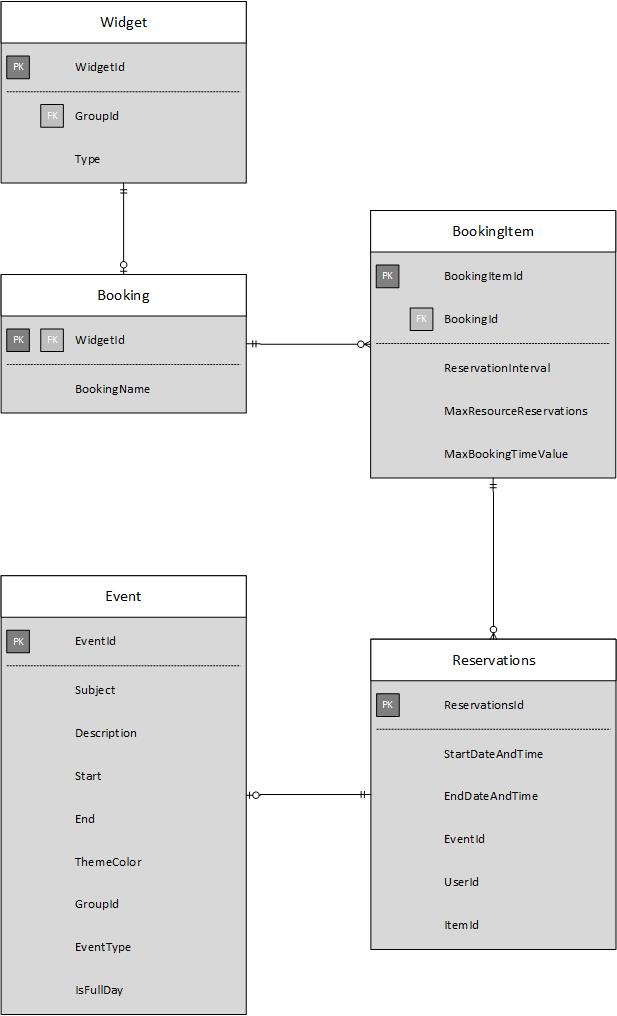
\includegraphics[width=0.5\linewidth]{01_Billeder/09_Arkitektur/Booking.jpg}
  \caption{ER diagram for booking system i databasen. For at kunne tilføje en ressource til et Booking-system, er det nødvendigt at et Booking-system skal have tilknyttet ressourcer(BookingItem). For at der kan foretages reservationer oprettes Reservations, hvor hver reservation tilhører ét BookingItem}
  \label{fig:Booking_ER}
\end{figure}

\subsection{Logical view}
De funktionaliteter der vurderes at blive anvendt oftest, skal være lettest tilgængelige. For at være let tilgængelige bør de kunne anvendes fra widgetten på Dashboardet. Her i rapporten vises der kun diagrammer der er relevante for de to US's som der beskrives i dette afsnit. Resten af diagrammerne kan findes i bilag.

\subsubsection{Tilføj/fjern/redigér ressource}
Arbejdet på de to US's der omhandler at oprette/slette/redigere en ressource, påbegyndes i 4. iteration. Der laves en indledende STM der beskriver hvilke views der kan navigeres rundt i for at oprette/fjerne ressource. Denne kan ses på figur \ref{fig:Booking_STMResource_Initial}
 
\begin{figure}[H]
  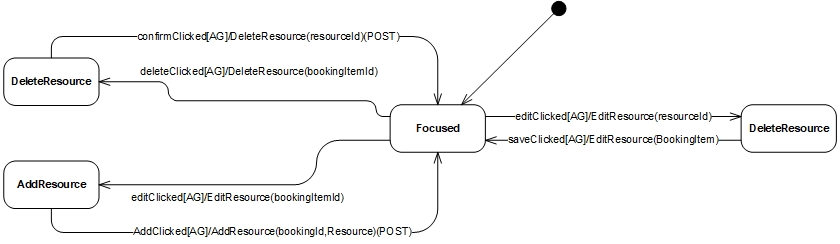
\includegraphics[width=1.0\linewidth]{01_Billeder/09_Arkitektur/STM_AddResource_Initial.jpg}
  \caption{STM fra 4. iteration viser hvordan der kan navigeres mellem forskellige views for at slette/redigere/oprette en ressource. Ordforklaring: AG - Access Granted. For at en bruger kan få adgang til Edit/Delete views, skal brugeren være admin}
  \label{fig:Booking_STMResource_Initial}
\end{figure}

Når widget containeren på dashboardet er klar til kunne anvendes, opdaterers arkitekturen for denne US. Dette gøres i iteration 6. Det vurderes at AddResource Viewet vil blive brugt oftere end Delete/Edit hvormed denne kan tilgås både fra \_Booking viewet og Focused viewet, hvor de to andre views kun kan tilgås fra Focused viewet. Desuden implementeres disse tre views nu som Pop-up vinduer. En STM der viser hvilke views den skal indeholde, og hvordan der kan navigeres mellem disse kan ses på figur \ref{fig:Booking_STMResource_Final}.  

\begin{figure}[H]
  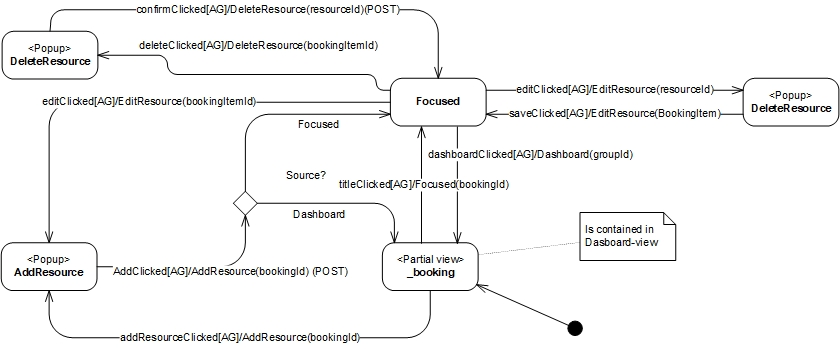
\includegraphics[width=1.0\linewidth]{01_Billeder/09_Arkitektur/STM_AddResource_Final.jpg}
  \caption{STM fra 6. iteration der viser hvordan der kan navigeres mellem forskellige views for at slette/redigere/oprette en ressource. Når POST funktionen kaldes efter der trykkes på 'Confirm', omdirigeres der til det view som pilen peger på. Ordforklaring: AG - Access Granted. For at en bruger kan få adgang til Edit/Delete views, skal brugeren være admin}
  \label{fig:Booking_STMResource_Final}
\end{figure}

\subsubsection{Opret gentagende reservation}
Arkitekturen af denne funktionalitet påbegyndes i iteration 5, efter det er blevet muligt at foretage en enkelt reservation af en ressource. For at kunne oprette en gentagende reservation er det blevet besluttet at skulle være en valgmulighed når der oprettes en enkelt reservation. En STM, fra iteration 5, der beskriver de mulige views som associeres med at oprette en gentagende reservation, kan ses på figur  \ref{fig:Booking_STMReservation_Initial}.   

\begin{figure}[H]
  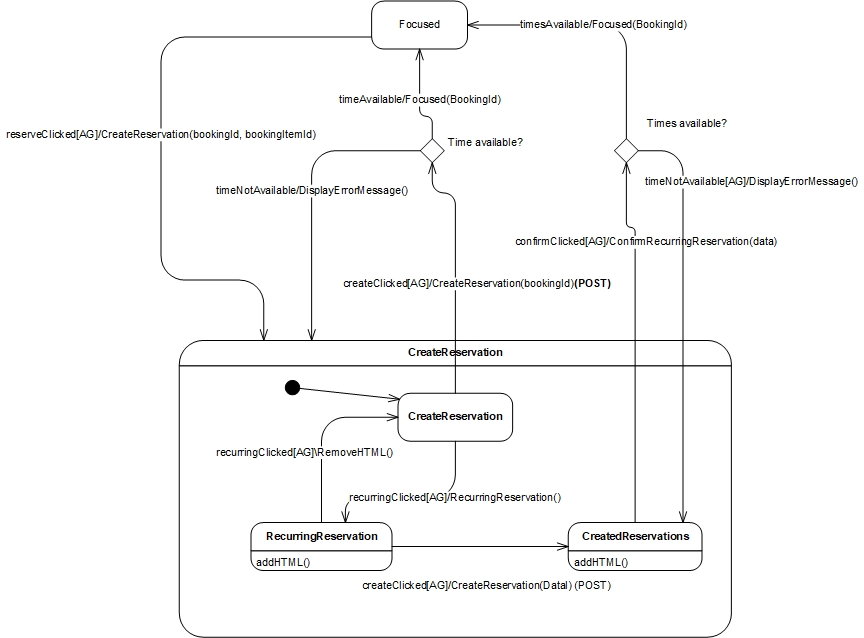
\includegraphics[width=1.0\linewidth]{01_Billeder/09_Arkitektur/STM_CreateReservation_Initial.jpg}
  \caption{STM der viser hvilke views der gør det muligt at oprette en gentagende reservation fra iteration 5. I CreateReservaition viewet repræsenterer der forskellige states, hvilket indold der vises. addHTML og removeHTML funktionerne viser hvornår der tilføjes/fjernes indhold. Ordforklaring: AG - AccessGranted}
  \label{fig:Booking_STMReservation_Initial}
\end{figure}
 Hvis der vælges at der skal foretages gentagende reservationer, hentes indhold fra serveren som indeholder valgmuligheder for at foretage gentagende reservationer. Efter brugeren trykker på create-knappen sendes information tilbage til serveren omkring brugerens ønskede reservationer. Serveren finder da ud af hvilke reservationer er mulige, og sender da denne information tilbage til klienten, som da vises på skærmen. Brugeren skal da bekræfte reservationerne. Afhængig af om tiderne stadig er ledige, omdirigeres til Focused viewet, eller der vises en fejlbesked.
Alle disse skridt er nødvendige for at sikre at der ikke kan foretages reservationer, hvor en ressource er reserveret af en anden bruger.

I 6. iteration, når widgetten containeren bliver klar, opdateres arkitekturen for denne US. Her laves siden hvor der foretages gentagende reservationer, om til et pop-up vindue. Desuden bliver det muligt at tilgå denne funktionalitet fra en Booking-widget fra dashboard. En STM der viser dette kan ses på figur \ref{fig:Booking_STMReservation_Final}. Den præcis samme funktionalitet er tilgængelig fra Focused viewet, men vises ikke her, da dette ville være overflødigt. 

\begin{figure}[H]
  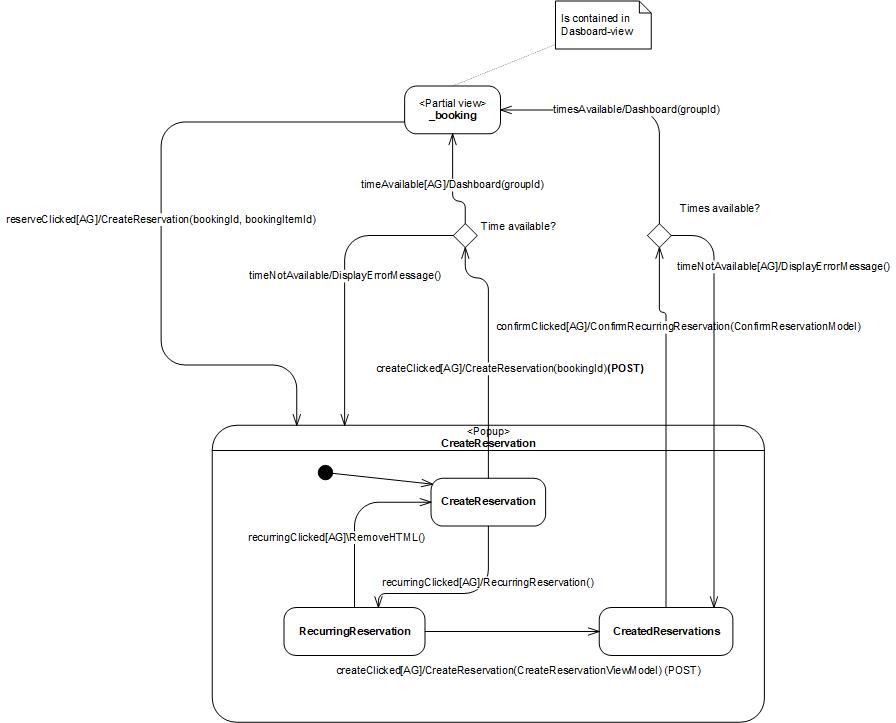
\includegraphics[width=1.0\linewidth]{01_Billeder/09_Arkitektur/STM_CreateReservationReport.jpg}
  \caption{STM der viser hvilke views der gør det muligt at oprette en gentagende reservation fra en Booking-widget i dashboardet for iteration 6. Når brugeren opretter de gentagende reservationer, omdirigeres atomatisk til den side som reservationerne blev foretaget fra.  Ordforklaring: AG - AccessGranted}
  \label{fig:Booking_STMReservation_Final}
\end{figure}

Restriktionen om at allerede reserveret ressource ikke skal kunne reserveres, går igen i hele arkitekturen for Booking. STM's for den resterende arkitektur kan findes i bilag. 
\valdemar{Skal indsætte reference til bilag}










